\documentclass[12pt,a4paper]{article}

% --- Packages ---
\usepackage[utf8]{inputenc}
\usepackage[margin=1in]{geometry}
\usepackage{graphicx}
\usepackage{amsmath}
\usepackage{amsfonts}
\usepackage{amssymb}
\usepackage{booktabs}
\usepackage{hyperref}
\usepackage{listings}
\usepackage[table]{xcolor}
\usepackage{titlesec}
\usepackage{tikz}
\usetikzlibrary{shapes.geometric, arrows, positioning}
\usepackage{float}
\usepackage{tabularx}

% --- Color Definitions ---
\definecolor{primary}{HTML}{333333}
\definecolor{darkblue}{HTML}{111111}
\definecolor{lightgray}{HTML}{F3F4F6}
\definecolor{tableheader}{HTML}{1B365D}
\definecolor{codegray}{rgb}{0.5,0.5,0.5}
\definecolor{codegreen}{rgb}{0,0.6,0}
\definecolor{codeblue}{rgb}{0.1,0.1,0.1}

% --- Listings Config ---
\lstset{
    backgroundcolor=\color{lightgray},
    basicstyle=\ttfamily\small,
    breakatwhitespace=false,
    breaklines=true,
    captionpos=b,
    commentstyle=\color{codegreen},
    keepspaces=true,
    keywordstyle=\color{codeblue},
    numbers=left,
    numbernumber=1,
    numbersep=5pt,
    numberstyle=\tiny\color{codegray},
    showspaces=false,
    showstringspaces=false,
    showtabs=false,
    tabsize=2,
    frame=single,
    rulecolor=\color{gray!30}
}

% --- Header/Footer Customization ---
\usepackage{fancyhdr}
\pagestyle{fancy}
\fancyhf{}
\fancyhead[L]{Software Process Management}
\fancyhead[R]{Assignment 01 Project Report}
\fancyfoot[C]{\thepage}

\titleformat{\section}
  {\normalfont\Large\bfseries\color{darkblue}}{\thesection}{1em}{}

\titleformat{\subsection}
  {\normalfont\large\bfseries\color{primary}}{\thesubsection}{1em}{}

% --- Begin Document ---
\begin{document}

% ==========================================
% COVER PAGE
% ==========================================
\begin{titlepage}
    \centering
    \vspace*{0.5cm}
    
\includegraphics[width=3.5cm]{uni_logo.png}\par
    \vspace{1.2cm}
    
    {\large\bfseries Assignment 01 Project Report\par}
    \vspace{0.2cm}
    {\large\bfseries Group: 07\par}
    
    \vspace{1.5cm}
    {\Huge \bfseries DevOps-Driven \\[0.3cm] Learning Management System (LMS) \par}
    \vspace{1.5cm}
    {\large\bfseries Project Team Members\par}
    \vspace{0.4cm}
    {\small
    \begin{tabular}{|l|l|l|}
        \hline
        \textbf{Index Number} & \textbf{Student Name} & \textbf{Assigned Role} \\
        \hline
        FC222011 & M.W.S. Ekanayaka & Developer \\
        \hline
        FC222033 & S.T. Rahman & Frontend Dev \\
        \hline
        FC222028 & U.S. Ravihara & DevOps Engineer \\
        \hline
        FC222026 & O.P.S. Perera & QA Engineer \\
        \hline
        FC222002 & L.R. Thuduwege & Product Owner \\
        \hline
        FC222037 & S.M.S.Y. Wickramarathna & Scrum Master \\
        \hline
    \end{tabular}
    }
    
    \vfill
    
    {\large\bfseries CSE3032 -- Software Process Management -- July 2026\par}
    \vspace{0.5cm}
    {\large Faculty of Computing\par}
    \vspace{0.2cm}
    {\large University of Sri Jayewardenepura\par}
    
\end{titlepage}

\newpage
\tableofcontents
\newpage

% ==========================================
% PROJECT LINKS
% ==========================================
\section*{Project Links}
\begin{tabular}{ll}
    \textbf{GitHub Repository:} & \url{https://github.com/SeniduRavihara/spm-lms} \\[6pt]
    \textbf{Live Application:}  & \url{http://134.185.84.132/} \\
\end{tabular}
\vspace{1cm}

% ==========================================
% 1. INTRODUCTION
% ==========================================
\section{Introduction}
The use of digital technologies in today’s education system has moved from being a nice-to-have to becoming an absolute requirement. The Learning Management System (LMS) becomes the software platform that supports this process of making the shift toward digitalization. An LMS becomes a common ground where educators can prepare and deliver the course content and students can access the resources and monitor their educational progress.

This product, called \textbf{SPM LMS}, is a high-quality full-stack Learning Management System aimed at solving two major problems in today’s digitalized classroom – a rich dashboard for the students and syllabus authoring functionality for the teachers.

\subsection{Tech Stack \& Architecture}
The system uses an architecture as follows for better performance, separation of concerns, and easy deployment:
\begin{itemize}
    \item \textbf{Front-end:} For the frontend we use react feamrwork called Nextjs, and the taledwindcss used for styling, and framermotion library for the animation
    \item \textbf{Back-end:} We used the TypeScript programming language to create our back-end and integrated it with REST API and with the Express.js framework. This takes care of routing, sessions, database connectivity and JWT auth. 
    \item \textbf{Database and ORM:} For database we chose serverless Neon PostgreSQL Database. We chose Prisma ORM for migration and query compilation.
    \item \textbf{DevOps:} Our whole application is deployed within Docker containers with the help of Docker Compose. The reverse proxy Nginx is deployed in the same cheap Oracle Cloud VPS having 1 GB of RAM, costing \$5 per month.
\end{itemize}

% ==========================================
% 2. PROBLEM DEFINITION
% ==========================================
\section{Project Goals \& Problem Definition}
Most schools and colleges use some kind of LMS today. However, setting them up, configuring them, and keeping hosting costs low is still a massive technical challenge. We focused on solving these specific issues:

\begin{enumerate}
    \item \textbf{Disconnection Between User Experience:} Most LMS systems currently have messy, non-responsive, and unattractive user interface systems, which result in disengaged students, confusion with respect to the course progression, and more work for teachers who have to deal with sophisticated content authoring systems.
    \item \textbf{Costly Hosting Environment:} There is a huge cost associated with hosting a full-stack web application. Every time frameworks like Next.js and Express.js are hosted on low-cost servers, there are server crash problems due to memory exhaustion. Thus, there needs to be a way to make these apps run efficiently on cheap servers.
    \item \textbf{Vulnerabilities of Database and Port Exposure:} Direct exposure of raw database ports (PostgreSQL) and application ports to the Internet introduces huge security risks. There is a need to develop routing that can proxy the external ports through one specific port (port 80).
    \item \textbf{Manual, Slow Deployments:} Uploading files manually over SSH, compiling code directly on the server, and restarting services by hand is slow and causes downtime. A single typo can break the production app. We needed a workflow to build, test, and release code automatically.
\end{enumerate}

% ==========================================
% 3. SOFTWARE PROCESS MODEL USED
% ==========================================
\section{Our Software Development Model}
The DevOps Driven Learning Management System (LMS) was developed based on the Agile Scrum software process model, incorporating DevOps practices. This approach was chosen because it permits continuous development, team collaboration and regular software delivery. Agile is different from traditional development models in that it allows the project to evolve through small iterations and it allows changes in requirements for the development process .

DevOps was another layer of improvement to the development process, enabling continuous integration, automated testing and better deployment. The team used agile and DevOps to speed up the delivery of new features, while maintaining software quality and reducing the time spent on identifying and fixing bugs.

\subsection{Advantages of the Selected Process Model}
Several advantages were gained in the development of the Learning Management System with the combination of Agile Scrum and DevOps. Breaking the project into several sprints made the large development tasks manageable and allowed team members to work on different modules at the same time. Constant feedback from the supervisor enabled the system to meet project objectives while allowing improvements to be made during development.

The quality of software improved by implementing DevOps practices, which fostered frequent integration, continuous testing, and automated deployment. These practices helped to reduce integration problems, reduce the number of errors made during deployment and allowed the team to identify problems earlier than traditional development approaches.

\subsection{Challenges Encountered}
There were a number of benefits of the selected process model; however, there were several challenges encountered during the project. Good communication and version control were required to help coordinate the development activities of several team members. Sometimes merge conflicts happened when different developers changed the same files at the same time.

In the early days of the project, we also had to put in more effort to set up Continuous Integration workflows. Also, writing automated tests for all features was time-consuming due to the limited time of the project. In spite of these challenges, the Agile Scrum and DevOps approach helped the team to successfully complete the project with an acceptable quality of the software.

% ==========================================
% 4. AGILE/SCRUM PRACTICES
% ==========================================
\section{How We Managed Sprints}
We ran our development in short sprint cycles, assigning specific roles and keeping to a tight schedule of ceremonies to keep the team moving forward.

\subsection{Roles in Scrum}
\begin{itemize}
    \item \textbf{Product Owner:} Managed the backlogs. They created user stories to ensure that all features we create would serve their purpose.
    \item \textbf{Scrum Master:} Keep the schedule align with the development while track and assign the issus like CORS error we faced, and the docker composer connection issu
    \item \textbf{Development Team:} The rest of the team was working on the project. We created the UI using Next.js, created Express API, Prisma schemas, and used Jest.
\end{itemize}

\subsection{Sprint Routines}
\begin{enumerate}
    \item \textbf{Sprint Planning Meetings:} Before we started the sprint, we would go through the backlog and select which tasks we will do. We had estimates in story points, and we set a realistic goal for ourselves.
    \item \textbf{Daily Standup:} we had 10 mins meeitngs everyday , everybody shared what they did in the privious day, what they planed to do next day, and if there is anything holding them back due to bugs.
    \item \textbf{Sprint Reviews:} At the end, we review our frontend dashboard and the backend api routes to ensure everything was working correcly as apected
    \item \textbf{Sprint Retrospective:} We went over our process after each release, which allowed us to find possible issues and bottlenecks, like slow Docker build times.
\end{enumerate}

\subsection{Sprint Breakdown}
\begin{figure}[H]
    \centering
    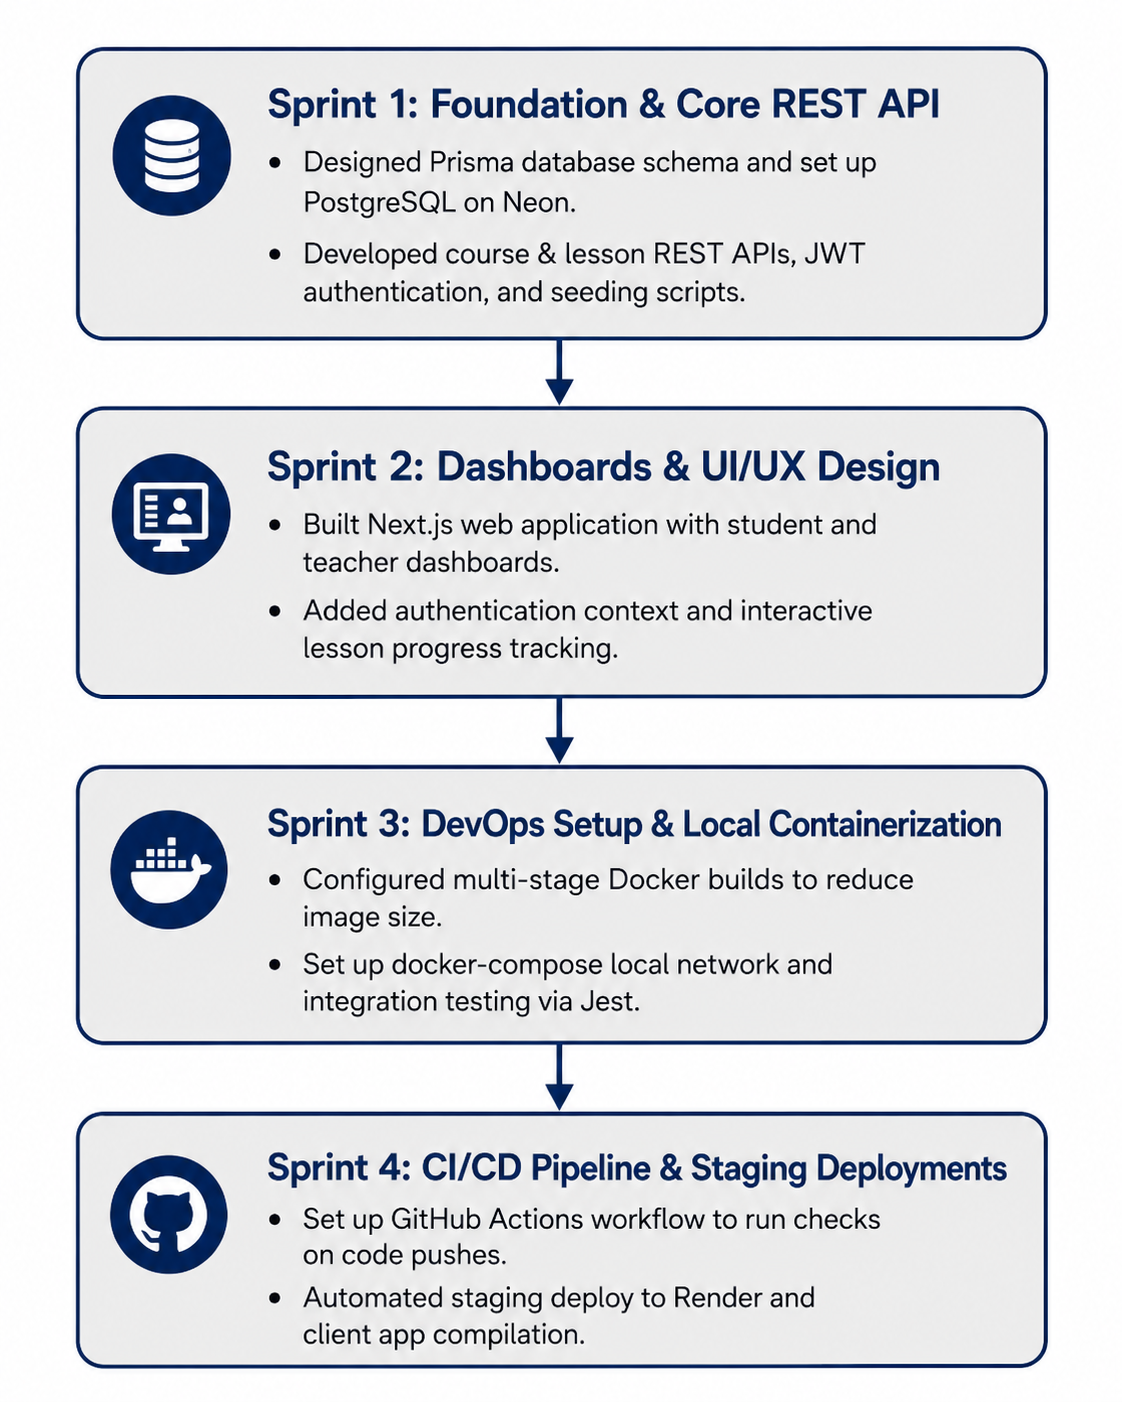
\includegraphics[width=0.9\textwidth]{sprint_timeline.png}
    \caption{Sprint Breakdown and Development Timeline}
    \label{fig:sprint_timeline}
\end{figure}

% ==========================================
% 5. GIT WORKFLOW
% ==========================================
\section{Git Workflow}
To support parallel development and maintain a stable codebase, the team adopted a structured branching strategy. Feature branches were merged into \texttt{main} after local verification.

\subsection{Git Branching Visualization}
Below is a conceptual representation of the Git branching strategy followed during development:

\begin{figure}[H]
    \centering
    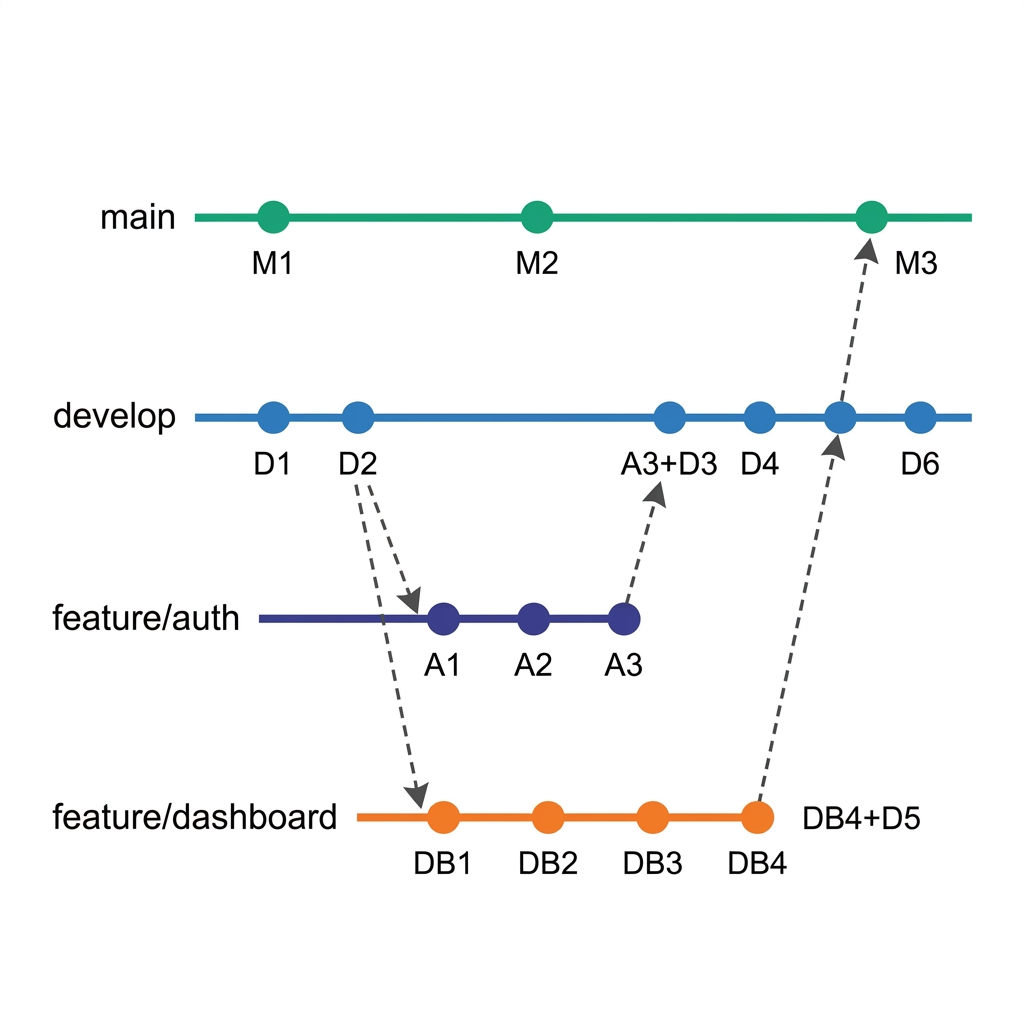
\includegraphics[width=0.8\textwidth]{git_workflow.png}
    \caption{Git Branching Strategy Flowchart (Git Flow)}
    \label{fig:git_workflow}
\end{figure}

\subsection{Key Workflow Rules}
\begin{enumerate}
    \item \textbf{Protected Main Branch:} Only stable, tested code goes into \texttt{main}. We block direct pushes to this branch to protect production.
    \item \textbf{Feature-specific Branches:} We create a separate branch for every feature or fix (like \texttt{feature/auth-jwt}). This keeps our work isolated while developing.
    \item \textbf{Pull Requests \& Reviews:} Before merging anything into \texttt{main} or \texttt{develop}, we open a Pull Request so other team members can review the changes.
\end{enumerate}

% ==========================================
% 6. CI/CD IMPLEMENTATION
% ==========================================
\section{CI/CD Automation}
We set up a CI pipeline using GitHub Actions to automate testing and prevent code regression. Everything is defined in \texttt{.github/workflows/ci.yml}, which triggers on every commit and pull request.

\subsection{CI Pipeline Lifecycle Flow}
\begin{figure}[H]
    \centering
    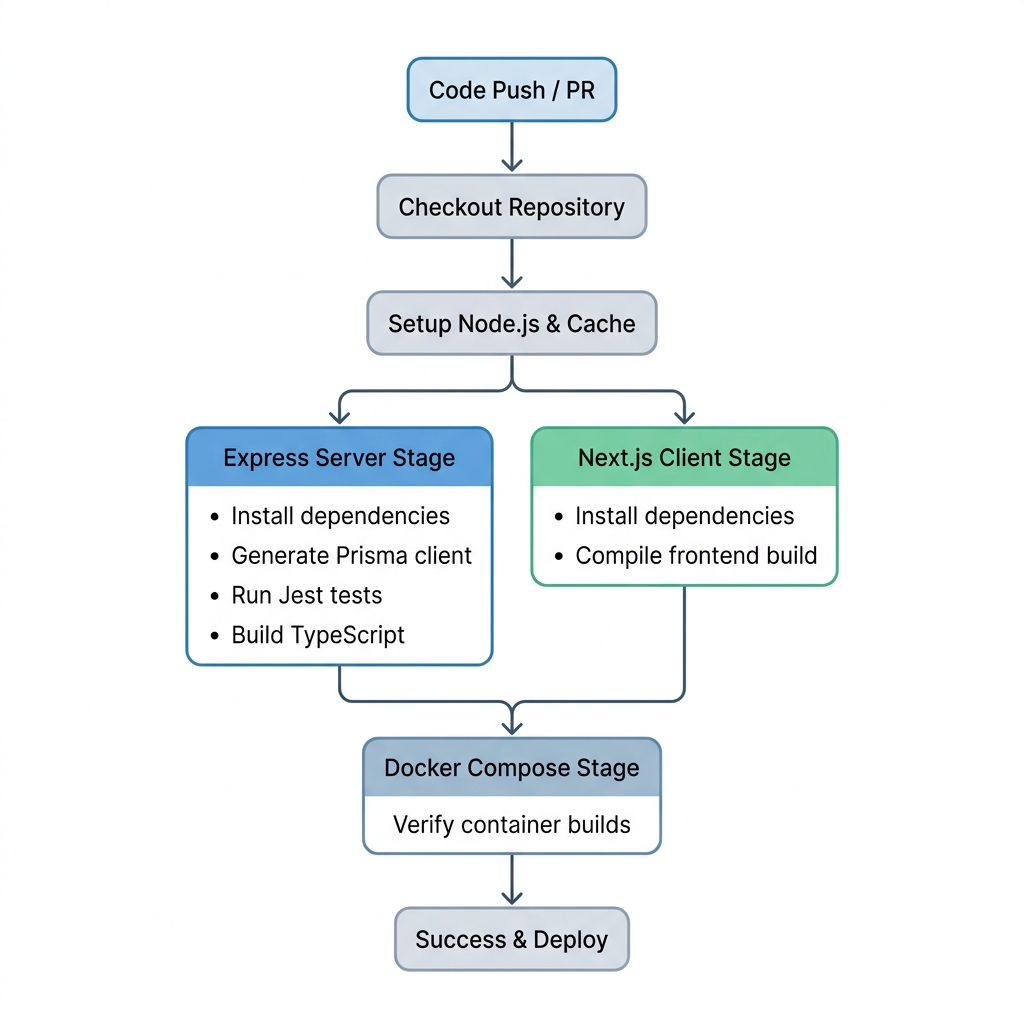
\includegraphics[width=0.8\textwidth]{ci_pipeline_flow.png}
    \caption{CI/CD Pipeline Lifecycle flowchart}
    \label{fig:ci_pipeline_flow}
\end{figure}

\subsection{CI Pipeline Workflow Details}
\begin{itemize}
    \item \textbf{Environment Setup:} Runs on the \texttt{ubuntu-latest} GitHub Actions runner.
    \item \textbf{Node.js Configuration:} Node.js v20 is installed, and npm caching is enabled to speed up dependency installations.
    \item \textbf{Express Backend Process:}
    \begin{itemize}
        \item Installs server dependencies using \texttt{npm ci}.
        \item Generates the Prisma Client: \texttt{npx prisma generate}.
        \item Executes backend integration tests using Jest and Supertest: \texttt{npm run test}.
        \item Builds the TypeScript project: \texttt{npm run build}.
    \end{itemize}
    \item \textbf{Next.js Frontend Process:} Installs client dependencies and compiles the frontend build.
    \item \textbf{Docker Validation:} Installs Docker Buildx and compiles the target docker-compose images to ensure container compatibility.
    \item \textbf{Continuous Deployment (CD) via SSH:} Triggered only on pushes to the \texttt{main} branch. It authenticates with the VPS using encrypted private keys stored in GitHub Repository Secrets, logs in via SSH, pulls the latest commit, and commands Docker Compose to rebuild and restart the target services.
\end{itemize}

\begin{figure}[H]
    \centering
    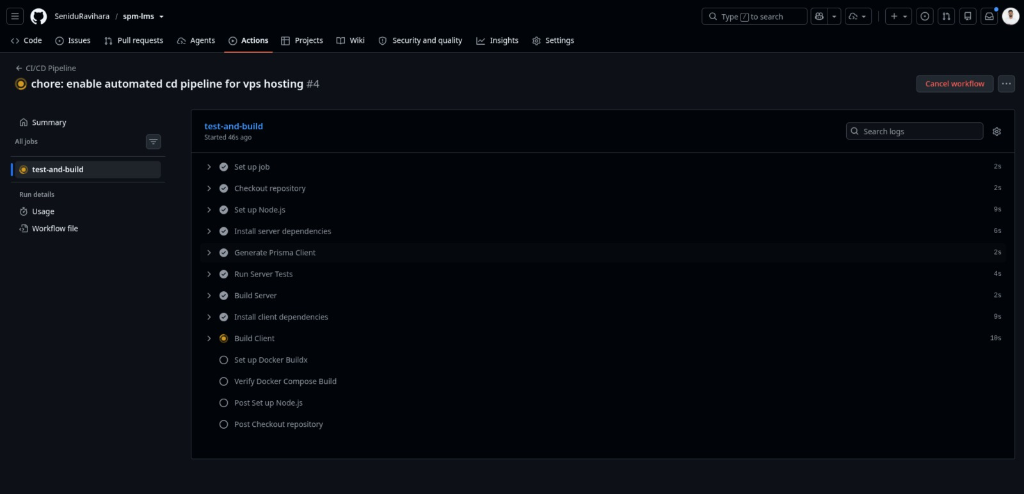
\includegraphics[width=0.9\textwidth]{pipeline_steps.png}
    \caption{GitHub Actions Pipeline Step-by-Step Execution Logs}
    \label{fig:pipeline_steps}
\end{figure}

\begin{figure}[H]
    \centering
    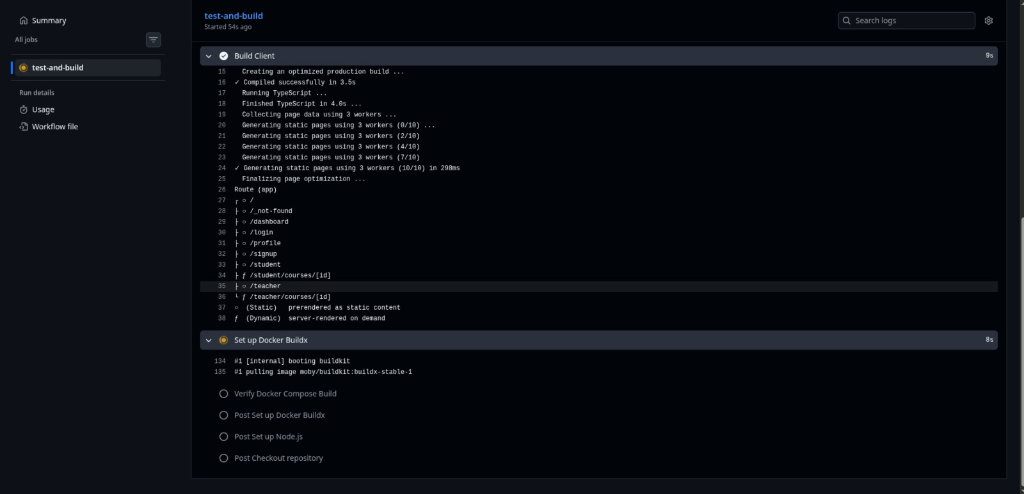
\includegraphics[width=0.9\textwidth]{client_build_logs.png}
    \caption{Next.js Frontend Production Build and Static Page Optimization Outputs}
    \label{fig:client_build_logs}
\end{figure}

% ==========================================
% 7. DOCKER USAGE
% ==========================================
\section{Docker Usage}
In order to provide consistency between the development environment, CI runners,
and the production server, Docker and Docker Compose were used to containerize
the application.

\subsection{Multi-Stage Docker Builds}
The application uses multi-stage builds for both frontend and backend in order to
make production images smaller.

\subsubsection{Backend (server/Dockerfile)}

\begin{figure}[H]
    \centering
    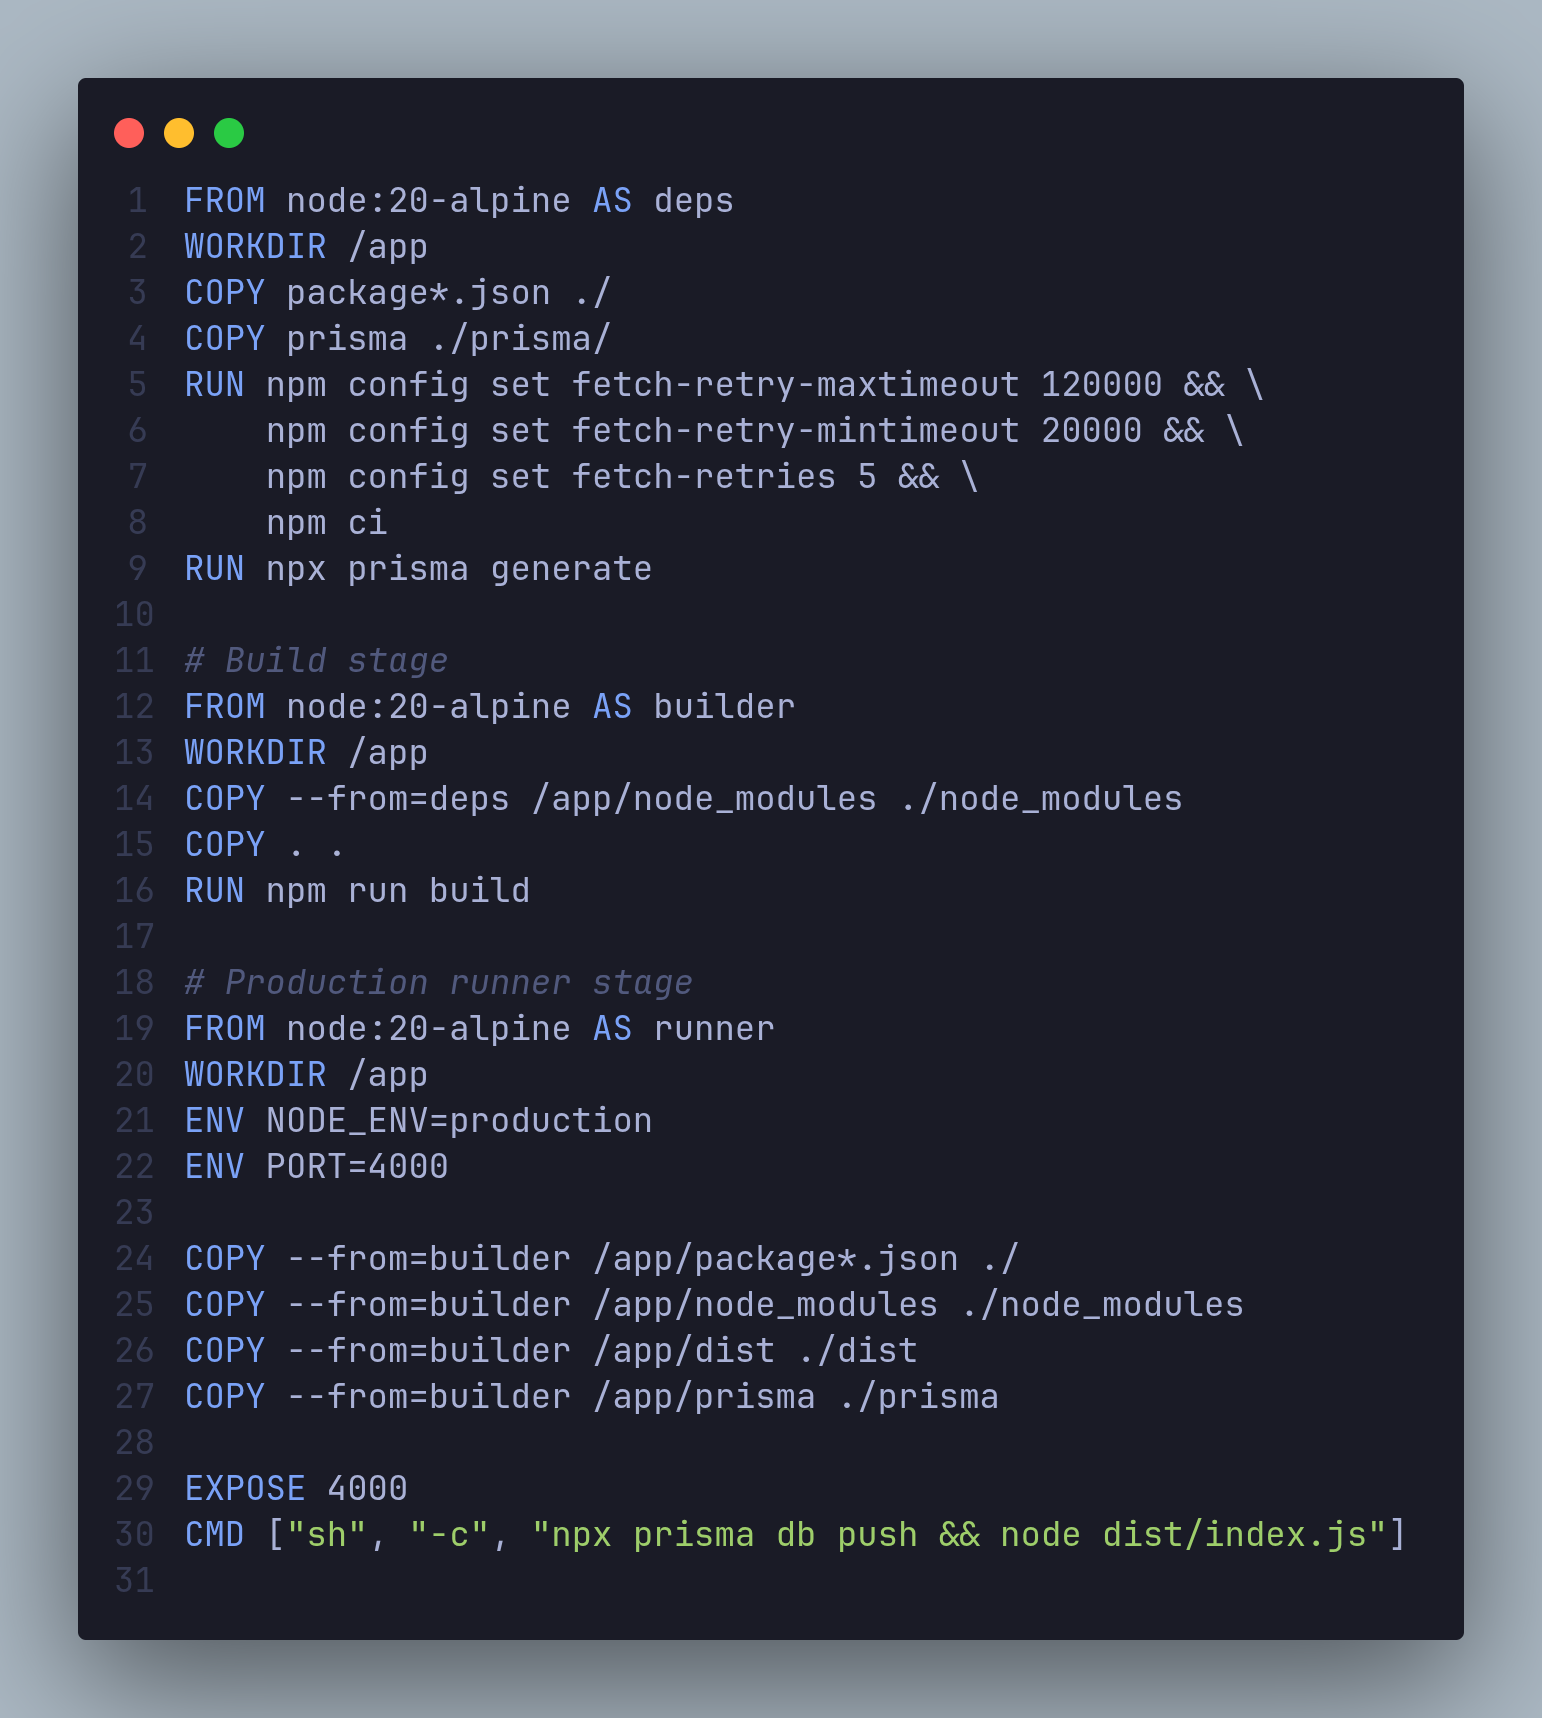
\includegraphics[width=0.9\textwidth]{code1.png}
    \caption{Multistage Dockerfile Configuration for Express Backend Service}
    \label{fig:backend_dockerfile}
\end{figure}

\subsubsection{Frontend (client/Dockerfile)}
Client application was also containerized, by copying the compiled .next folder in order
to make the target image smaller (from 1.5 GB to 250 MB).


% ==========================================
% 8. TESTING STRATEGY
% ==========================================
\section{Testing Strategy}
There was use of the testing methodology within the course of developing the software, where different aspects of the software were tested to ensure their efficiency. This involved an extensive process of unit testing, integration testing, and end-to-end testing. We managed to test different frontend and backend API routes to ensure that the system fulfills our requirements of performance and security.

\subsection{Backend Integration Testing (Jest \& Supertest)}
The following integration test suites have been developed:
\begin{itemize}
    \item Authentication (auth.test.ts): To validate password hashing, token valida-
tion, and structure of signup/login controllers.
    \item Courses (courses.test.ts): To validate CRUD operations, and ensures that
only users with teacher role are allowed to create new courses.
    \item Lessons (lessons.test.ts): Validates course syllabi structures.
    \item Student Progress (progress.test.ts): Validates lesson completion checklists,
and math operations for percent bar update.
\end{itemize}

\begin{figure}[H]
    \centering
    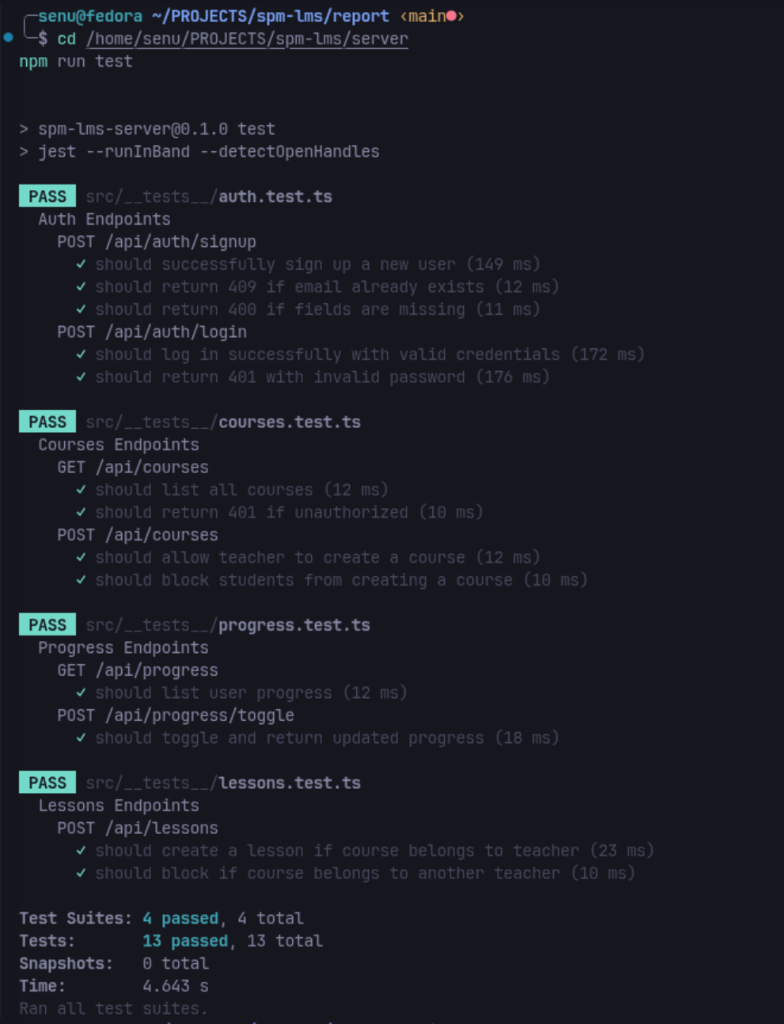
\includegraphics[width=0.55\textwidth]{test_results.png}
    \caption{Successful integration tests for Express backend endpoints using Jest}
    \label{fig:test_results}
\end{figure}

\subsection{Detailed Test Cases}
In order to validate the correctness, reliability and security of the system, the follow-
ing test case suite was conducted. The list of test cases is provided in Table 2 below:

\begin{table}[H]
    \centering
    \caption{LMS Application Test Cases Matrix}
    \vspace{0.3cm}
    \begin{tabularx}{\textwidth}{|l|X|X|l|}
        \hline
        \textbf{ID} & \textbf{Test Case} & \textbf{Expected Result} & \textbf{Type} \\
        \hline
        TC-AUTH-01 & Login with correct username and password & Successfully authenticates user and returns a signed JWT token & Unit \\
        \hline
        TC-AUTH-02 & Access instructor course creation route with student role & HTTP 403 Forbidden error returned, protecting restricted resources & Integration \\
        \hline
        TC-AUTH-03 & Login with incorrect password credentials & HTTP 401 Unauthorized returned with an authentication failure message & Unit \\
        \hline
        TC-CRSE-01 & Create a new course with valid details as a teacher & Course entry successfully added to PostgreSQL database via Prisma & Integration \\
        \hline
        TC-LESS-01 & Fetch syllabus lessons for a course without being logged in & HTTP 401 Unauthorized returned, blocking public endpoint access & Integration \\
        \hline
        TC-PROG-01 & Toggle completion checkbox for a lesson in student course tracker & Successfully updates student's lesson completion state in database & Unit \\
        \hline
        TC-PROG-02 & Calculate progress percentage with 2 completed out of 10 lessons & Student dashboard accurately renders 20\% progress completion bar & Unit \\
        \hline
        TC-PORT-01 & Access live server on standard port 80 & Nginx reverse proxy forwards standard requests internally to port 3000 & E2E \\
        \hline
    \end{tabularx}
    \label{tab:test_cases}
\end{table}

% ==========================================
% 9. DEPLOYMENT PROCESS
% ==========================================
\section{Deployment Process}
The application was deployed using separate cloud services for the database, and unified containerized hosting for client and server.

\subsection{Database Hosting (NeonDB)}
The application uses NeonDB, a serverless PostgreSQL platform, for database hosting. Its key features include:
\begin{itemize}
    \item Serverless PostgreSQL infrastructure.
    \item Built-in connection pooling for improved performance.
    \item Automatic database schema synchronization using Prisma migrations.
\end{itemize}

\subsection{VPS Hosting \& Reverse Proxy (Nginx)}
The client and server run inside Docker containers on the Oracle Cloud VPS. The hosted application is publicly live and accessible at \url{http://134.185.84.132/}.

To make the application accessible on standard web ports without forcing the end user to enter container port numbers (such as \texttt{:3000} or \texttt{:4000}), Nginx was installed and configured as a reverse proxy on the VPS. Nginx listens on the public HTTP Port 80, intercepts incoming requests, and handles the internal port forwarding:
\begin{itemize}
    \item Standard page requests are forwarded internally to the Next.js Frontend container running on port \texttt{3000}.
    \item API requests directed to \texttt{/api} are forwarded internally to the Express Backend container running on port \texttt{4000}.
\end{itemize}
This setup ensures a seamless and secure access route for users while hiding raw container ports from the public internet.

\begin{figure}[H]
    \centering
    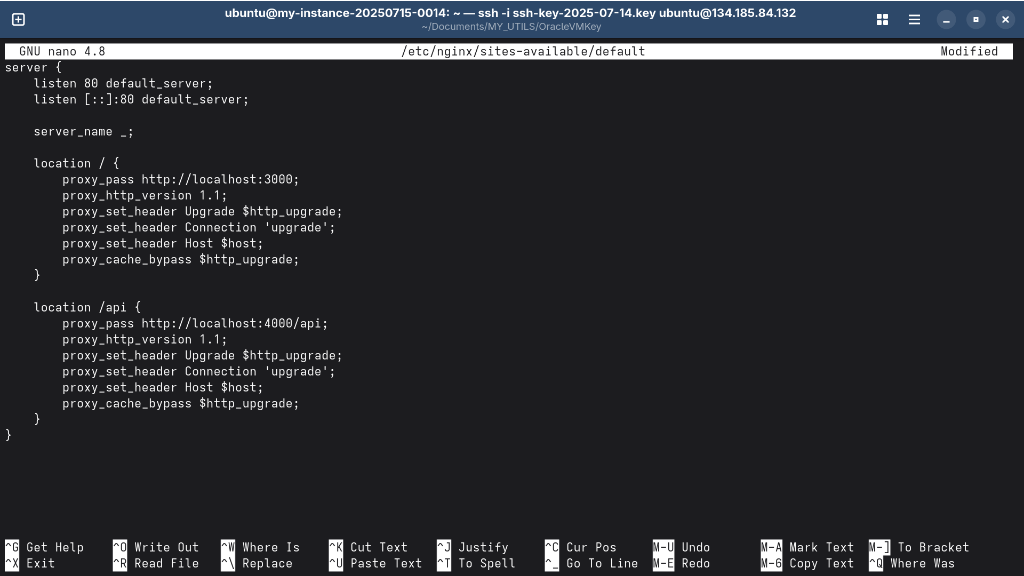
\includegraphics[width=\textwidth]{nginx_config.png}
    \caption{Nginx Reverse Proxy configuration routing Port 80 to Docker containers}
    \label{fig:nginx_config}
\end{figure}

\begin{figure}[H]
    \centering
    
\includegraphics[width=\textwidth]{live_website.png}
    \caption{The live production frontend application accessed via the VPS public IP address}
    \label{fig:live_website}
\end{figure}

\subsection{Automated Deployment Pipeline (GitHub Actions \& SSH)}
The entire deployment lifecycle is fully automated. Whenever code changes are pushed or merged to the \texttt{main} branch of the GitHub repository:
\begin{enumerate}
    \item The GitHub Actions runner executes standard tests and verifies container compilation.
    \item Upon build success, it initiates a secure SSH connection to the VPS (using port 22 with the SSH private key stored in GitHub repository secrets).
    \item It connects to the target directory on the VPS (\texttt{\textasciitilde/spm-lms}), pulls the latest code using \texttt{git pull origin main}, and rebuilds the containers in the background using \texttt{sudo docker compose up -d --build}.
\end{enumerate}
This ensures that the live production server is always up-to-date with minimal developer intervention and zero manual downtime.

\begin{figure}[H]
    \centering
    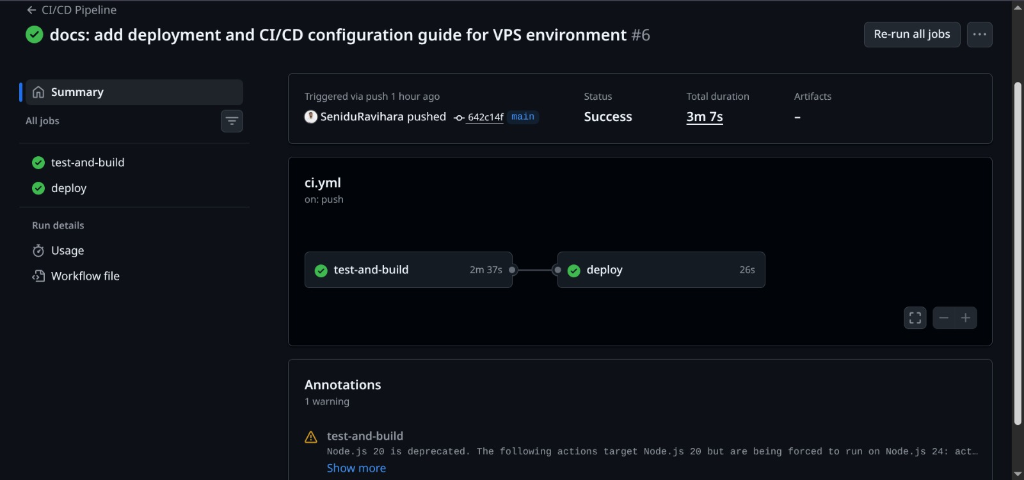
\includegraphics[width=0.9\textwidth]{pipeline_success.png}
    \caption{GitHub Actions Pipeline Execution Status Showing Successful Integration and Deploy Jobs}
    \label{fig:pipeline_success}
\end{figure}

% ==========================================
% 10. CHALLENGES FACED AND SOLUTIONS
% ==========================================
\section{Challenges Faced and Solutions}
\begin{enumerate}
    \item \textbf{Prisma Client Generation in CI Pipeline:}
    \begin{itemize}
        \item \textit{Problem:} CI tasks failed because the Prisma Client was missing during TypeScript compilation.
        \item \textit{Solution:} Added \texttt{npx prisma generate} immediately after dependency installation in both GitHub workflows and Docker builders.
    \end{itemize}
    \item \textbf{Large Docker Image Sizes:}
    \begin{itemize}
        \item \textit{Problem:} Initial Docker configuration produced images larger than 1.5 GB.
        \item \textit{Solution:} Implemented multi-stage builds using lightweight Alpine base images, dropping image size to under 250 MB.
    \end{itemize}
    \item \textbf{CORS and Docker Domain Configurations:}
    \begin{itemize}
        \item \textit{Problem:} Communication between frontend and backend containers failed due to cross-origin settings.
        \item \textit{Solution:} Standardized CORS config inside Express and supplied correct \texttt{NEXT\_PUBLIC\_API\_URL} build arguments.
    \end{itemize}
    \item \textbf{VPS Memory Constraints and Out-Of-Memory Crashes:}
    \begin{itemize}
        \item \textit{Problem:} The Next.js client-side production compilation process (\texttt{next build}) and running Docker daemons require more than the physical 1GB RAM provided by the free-tier VPS, leading to build crashes and process termination.
        \item \textit{Solution:} Configured a 4GB SSD-backed swapfile on the VPS as virtual memory. This prevents Out-Of-Memory (OOM) crashes by moving inactive processes to swap space during compilation spikes. Figure \ref{fig:htop_swap} shows the active system diagnostics under \texttt{htop}, verifying that the swap space is active and in use by the running containerized services (including next-server processes).
    \end{itemize}
\end{enumerate}

\begin{figure}[H]
    \centering
    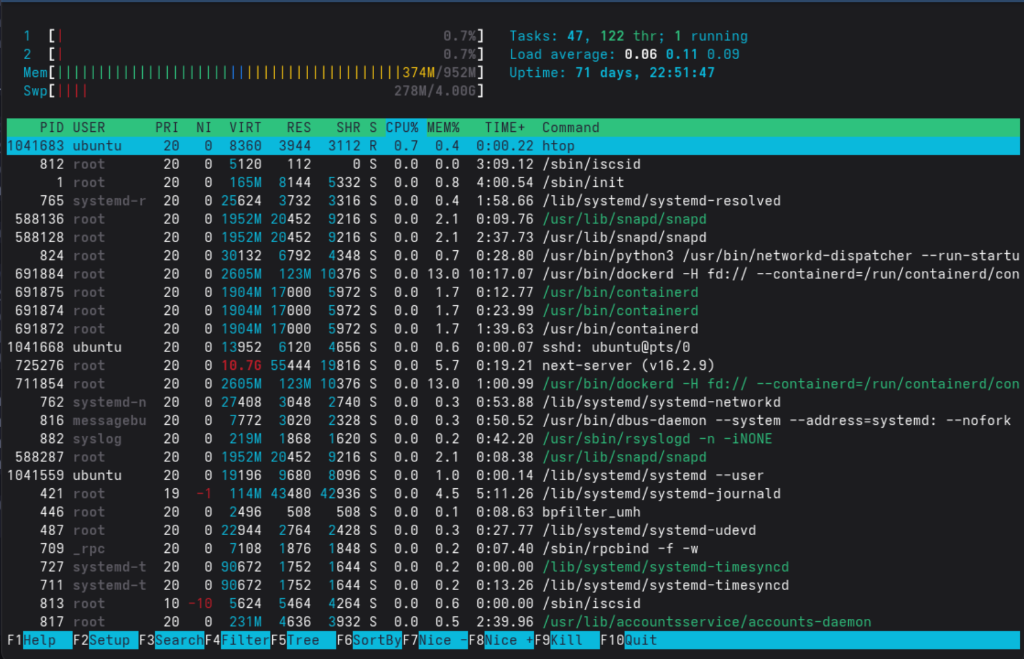
\includegraphics[width=0.9\textwidth]{htop_swap_metrics.png}
    \caption{Active VPS Diagnostics (htop) showing Swap Memory allocation and running Next.js server processes}
    \label{fig:htop_swap}
\end{figure}

% ==========================================
% 11. FUTURE IMPROVEMENTS
% ==========================================
\section{Future Improvements}
\begin{itemize}
    \item \textbf{AI for Personalized Learning:} Integrate recommendation systems that analyze students' study habits to deliver custom learning pathways.
    \item \textbf{AI-Powered Virtual Assistant:} Include a 24/7 chatbot to answer basic student queries and help debug technical system issues.
    \item \textbf{Advanced Learning Analytics:} Build interactive dashboards for teachers and admins to monitor aggregate student progress.
    \item \textbf{Video Conferencing Integrations:} Link the platform directly with Zoom or Google Meet API endpoints.
\end{itemize}

% ==========================================
% CONCLUSION
% ==========================================
\section{Conclusion}
The development and deployment of \textbf{SPM LMS} successfully demonstrate how modern software engineering principles, optimized containerized hosting, and automated DevOps practices can resolve the challenges of building a secure, performant, and cost-effective Learning Management System.

% ==========================================
% TEAM MEMBERS TABLE
% ==========================================
\section{Team Members \& Individual Contributions}

\begin{table}[H]
    \centering
    \caption{Team Members and Assigned Project Roles}
    \vspace{0.3cm}
    \begin{tabularx}{\textwidth}{|l|l|l|X|}
        \hline
        \textbf{Index Number} & \textbf{Student Name} & \textbf{Assigned Role} & \textbf{Key Contributions} \\
        \hline
        FC222011 & M.W.S. Ekanayaka & Developer & Backend API development, REST controllers \\
        \hline
        FC222033 & S.T. Rahman & Frontend Dev & Next.js portal UI, Framer Motion integration \\
        \hline
        FC222028 & U.S. Ravihara & DevOps Engineer & Docker, Nginx Proxy, swapfile memory setup \\
        \hline
        FC222026 & O.P.S. Perera & QA Engineer & Jest and Supertest integration tests \\
        \hline
        FC222002 & L.R. Thuduwege & Product Owner & Backlog management, Sprint planning \\
        \hline
        FC222037 & S.M.S.Y. Wickramarathna & Scrum Master & Daily standups, resolving Docker-CORS blockers \\
        \hline
    \end{tabularx}
\end{table}

\end{document}
